\documentclass[a4paper]{beamer}%handout


\usepackage{listings}
\usepackage{color}
 
\definecolor{codegreen}{rgb}{0,0.6,0}
\definecolor{codegray}{rgb}{0.5,0.5,0.5}
\definecolor{codepurple}{rgb}{0.58,0,0.82}
\definecolor{backcolour}{rgb}{0.95,0.95,0.92}


%% Add Matlab code
\usepackage{mcode}
%% Add Matlab code end


%% Add watermarks
%\usepackage{draftwatermark}
%% Add watermarks end
\usepackage[utf8]{inputenc}
\usepackage{multicol}
\usepackage{url}
\usepackage{hyperref}
\hypersetup{
	colorlinks=true,
	linkcolor=cyan,          % color of internal links (change box color with linkbordercolor)
    citecolor=green,        % color of links to bibliography
    filecolor=magenta,      % color of file links
    urlcolor=cyan           % color of external links
	}

\graphicspath{{img/}}

\mode<presentation> {

%\usetheme{default}%yes % use %\frametitle in all slides recommended
%\usetheme{AnnArbor}%no
%\usetheme{Antibes} %yes %favorite
%\usetheme{Bergen} %no
%\usetheme{Berkeley} %no
%\usetheme{Berlin} %no
%\usetheme{Boadilla} %yes % good use of paper space
%\usetheme{CambridgeUS} %yes %favorite %use %\frametitle recommended
%\usetheme{Copenhagen}%yes%noframetitle
%\usetheme{Darmstadt}%no
%\usetheme{Dresden}
%\usetheme{Frankfurt}
%\usetheme{Goettingen}
%\usetheme{Hannover}
%\usetheme{Ilmenau}%no
%\usetheme{JuanLesPins}
%\usetheme{Luebeck}
%\usetheme{Madrid}
%\usetheme{Malmoe}
%\usetheme{Marburg}
%\usetheme{Montpellier}
%\usetheme{PaloAlto}
%\usetheme{Pittsburgh}%no
%\usetheme{Rochester}%no
%\usetheme{Singapore}%yees
%\usetheme{Szeged}%no
%\usetheme{Warsaw}%no

% As well as themes, the Beamer class has a number of color themes
% for any slide theme. Uncomment each of these in turn to see how it
% changes the colors of your current slide theme.

%\usecolortheme{albatross}
%\usecolortheme{beaver}
%\usecolortheme{beetle}
%\usecolortheme{crane}
\usecolortheme{dolphin}
%\usecolortheme{dove}
%\usecolortheme{fly}
%\usecolortheme{lily}
%\usecolortheme{orchid}
%\usecolortheme{rose}
%\usecolortheme{seagull}
%\usecolortheme{seahorse}
%\usecolortheme{whale}
%\usecolortheme{wolverine}

\setbeamertemplate{footline} % To remove the footer line in all slides uncomment this line
%\setbeamertemplate{footline}[page number] % To replace the footer line in all slides with a simple slide count uncomment this line

\setbeamertemplate{navigation symbols}{} % To remove the navigation symbols from the bottom of all slides uncomment this line
}

%----------------------------------------------------------------------------------------
%	NEW COMMANDS
%----------------------------------------------------------------------------------------

\newcommand{\Conv}{\mathop{\scalebox{1.5}{\raisebox{-0.2ex}{$\ast$}}}}%
%\linespread{1.3}

%----------------------------------------------------------------------------------------
%	TITLE PAGE
%----------------------------------------------------------------------------------------

\title[Introduction]{Digital Image Processing} % The short title appears at the bottom of every slide, the full title is only on the title page

\author{Prof. Tiago Vieira} % Your name
\institute[UFAL] % Your institution as it will appear on the bottom of every slide, may be shorthand to save space
{
Universidade Federal de Alagoas \\ % Your institution for the title page
\medskip
\textit{tvieira@ic.ufal.br} % Your email address
}
\date{\today} % Date, can be changed to a custom date


%----------------------------------------------------------------------------------------
%	TITLE PAGE
%----------------------------------------------------------------------------------------

\subtitle{Image Formation -- Part II}

%------------------------------------------------

\begin{document}

%------------------------------------------------

\begin{frame}
\titlepage % Print the title page as the first slide
\end{frame}

%------------------------------------------------

\begin{frame}{Contents}
\setcounter{tocdepth}{1}
\tableofcontents
\end{frame}

%----------------------------------------------------------------------------------------
%	PRESENTATION SLIDES
%----------------------------------------------------------------------------------------

\section{Recap}

\section{Quick geometry recap}

\begin{frame}
\frametitle{Quick geometry recap}
\begin{itemize}
\item Some familiar concepts from geometry:
\begin{itemize}
\item Euclidean plane.
\begin{itemize}
\item A non-curved space where the rules of Euclidean geometry apply.
\end{itemize}
\item Cartesian coordinates.
\begin{itemize}
\item Distances to a point with respect to the origin and measured along orthogonal axes.
\end{itemize}
\end{itemize}
\end{itemize}
\begin{figure}[!h]
\centering
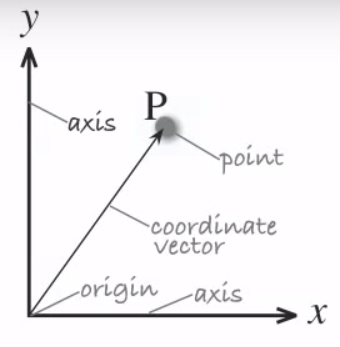
\includegraphics[width=.3\textwidth]{axes}
\end{figure}
\end{frame}

\begin{frame}
\frametitle{Homogeneous coordinates}
\begin{columns}
\begin{column}{.5\textwidth}
\begin{itemize}
\item Cartesian $\mapsto$ Homogeneous:
\end{itemize}
\[
\begin{array}{cc}
\textbf{P} = \left ( x, y \right ) & \tilde{\textbf{P}} = \left ( x, y, 1 \right ) \\
\textbf{P} \in \mathbb{R}^2 & \tilde{\textbf{P}} \in \mathbb{P}^2
\end{array}
\]
\begin{itemize}
\item Homogeneous $\mapsto$ Cartesian:
\end{itemize}
\[
\begin{array}{cc}
\tilde{\textbf{P}} = \left ( \tilde{x}, \tilde{y}, \tilde{z} \right ) \mapsto \textbf{P} = \left ( x, y \right )
\end{array}
\]
where
\[
x = \tilde{x}/\tilde{z},\ \ y = \tilde{y}/\tilde{z}.
\]
\end{column}
\begin{column}{.5\textwidth}
\begin{figure}[!h]
\centering
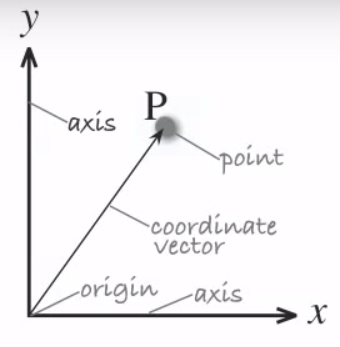
\includegraphics[width=\textwidth]{axes}
\end{figure}
\end{column}
\end{columns}
\begin{block}{In homogeneous coordinates}
Lines and points are duals!
\end{block}
\end{frame}

%\begin{frame}
%\frametitle{Homogeneous coordinates}
%\begin{block}{In homogeneous coordinates}
%Lines and points are duals!
%\end{block}
%\end{frame}
%
%\begin{frame}
%\frametitle{A line in homogeneous form}
%\begin{columns}
%\begin{column}{.5\textwidth}
%\begin{figure}[!h]
%\centering
%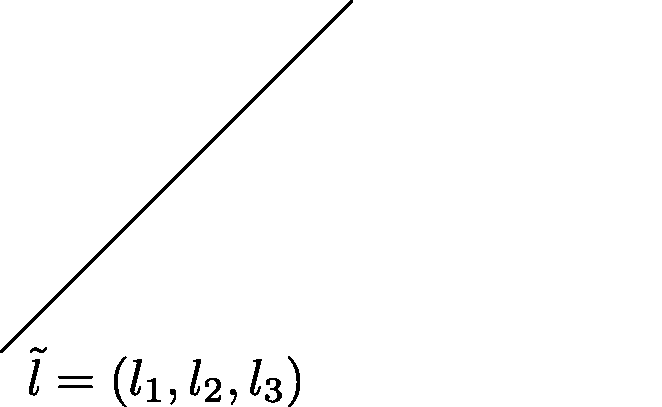
\includegraphics[width=\textwidth]{line0}
%\end{figure}
%\end{column}
%\begin{column}{.5\textwidth}
%
%\end{column}
%\end{columns}
%\end{frame}
%
%\begin{frame}
%\frametitle{A line in homogeneous form}
%\begin{columns}
%\begin{column}{.5\textwidth}
%\begin{figure}[!h]
%\centering
%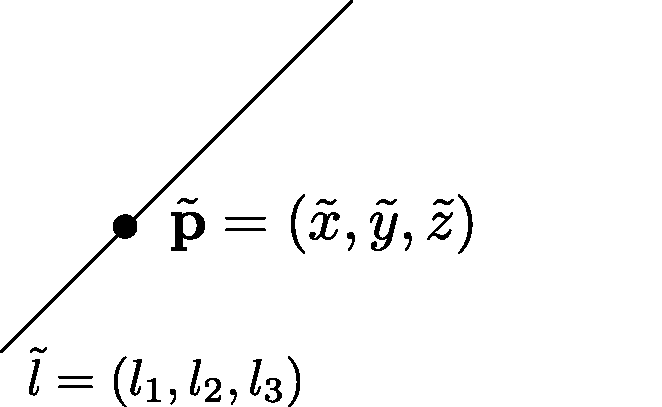
\includegraphics[width=\textwidth]{line1}
%\end{figure}
%\end{column}
%\begin{column}{.5\textwidth}
%
%\end{column}
%\end{columns}
%\end{frame}
%
%\begin{frame}
%\frametitle{A line in homogeneous form}
%\begin{columns}
%\begin{column}{.5\textwidth}
%\begin{figure}[!h]
%\centering
%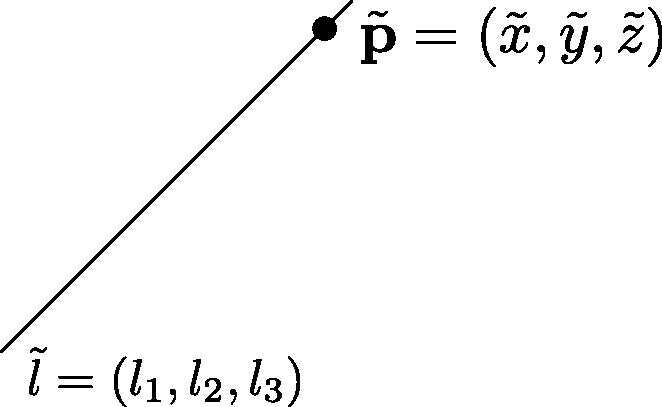
\includegraphics[width=\textwidth]{line2}
%\end{figure}
%\end{column}
%\begin{column}{.5\textwidth}
%A line is defined as a set of all points for which the dot product between the line and the point is equal to zero, ie.,
%\[
%\tilde{l}^{T} \tilde{\textbf{p}}=0
%\]
%\begin{itemize}
%\item This is the \textit{point equation of a line}.
%\item This form allows to treat the vertical case, in contrast with $y=ax+b$, where $a\mapsto \infty$.
%\end{itemize}
%\end{column}
%\end{columns}
%\end{frame}
%
%\begin{frame}
%\frametitle{Line joining points}
%\begin{columns}
%\begin{column}{.5\textwidth}
%\begin{figure}[!h]
%\centering
%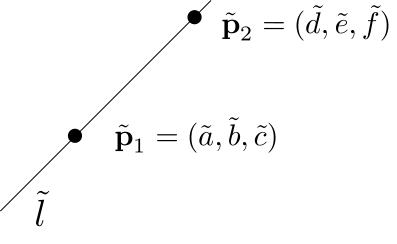
\includegraphics[width=\textwidth]{lineJoiningPoints}
%\end{figure}
%\end{column}
%\begin{column}{.5\textwidth}
%\[
%\tilde{l} = \tilde{\textbf{p}}_{1} \times \tilde{\textbf{p}}_2
%\]
%\end{column}
%\end{columns}
%\end{frame}
%
%\begin{frame}
%\frametitle{Intersecting lines}
%\begin{columns}
%\begin{column}{.5\textwidth}
%\begin{figure}[!h]
%\centering
%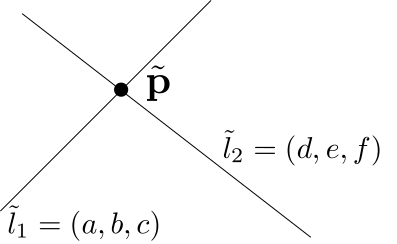
\includegraphics[width=\textwidth]{intersectingLines}
%\end{figure}
%\end{column}
%\begin{column}{.5\textwidth}
%Line equation of a point:
%\[
%\tilde{\textbf{p}} = \tilde{l}_{1} \times \tilde{l}_2
%\]
%\end{column}
%\end{columns}
%\end{frame}

\section{Pin-hole in homogeneous form}

\begin{frame}
\frametitle{Pin-hole in homogeneous form}
\[
\left (
\begin{array}{c}
\tilde{x}\\
\tilde{y}\\
\tilde{z}
\end{array}
\right )
=
\left (
\begin{array}{cccc}
f & 0 & 0 & 0 \\
0 & f & 0 & 0 \\
0 & 0 & 1 & 0
\end{array}
\right )
\left (
\begin{array}{c}
X \\
Y \\
Z \\
1
\end{array}
\right )
\]
I.e.,
\[
\tilde{x} = fX,\ \ \tilde{y} = fY,\ \ \tilde{z} = Z.
\]
As before:
\[
\left ( x = \tilde{x}/\tilde{z},\ \ y = \tilde{y}/\tilde{z}\right ) = \left ( x = \dfrac{fX}{Z},\ \ y = \dfrac{fY}{Z}\right )
\]
\begin{itemize}
\item Perspective transformation, with the divide by $Z$ is \textbf{linear} in homogeneous coordinate form.
\end{itemize}
\end{frame}

\begin{frame}
\frametitle{Pin-hole in homogeneous form}
\[
\left (
\begin{array}{c}
\tilde{x}\\
\tilde{y}\\
\tilde{z}
\end{array}
\right )
=
\left (
\begin{array}{cccc}
f & 0 & 0 & 0 \\
0 & f & 0 & 0 \\
0 & 0 & 1 & 0
\end{array}
\right )
\left (
\begin{array}{c}
X \\
Y \\
Z \\
1
\end{array}
\right )
\]
%
\[
\left (
\begin{array}{c}
\tilde{x}\\
\tilde{y}\\
\tilde{z}
\end{array}
\right )
=
\underbrace{
\left (
\begin{array}{cccc}
1 & 0 & 0 & 0 \\
0 & 1 & 0 & 0 \\
0 & 0 & 1 & 0
\end{array}
\right )
}_{3D \mapsto 2D}
\underbrace{
\left (
\begin{array}{cccc}
f & 0 & 0 & 0 \\
0 & f & 0 & 0 \\
0 & 0 & 1 & 0 \\
0 & 0 & 0 & 1
\end{array}
\right )
}_{\text{scaling/zooming}}
\left (
\begin{array}{c}
X \\
Y \\
Z \\
1
\end{array}
\right )
\]
\end{frame}

\begin{frame}
\frametitle{Central Projection Model}
\begin{figure}[!h]
\centering
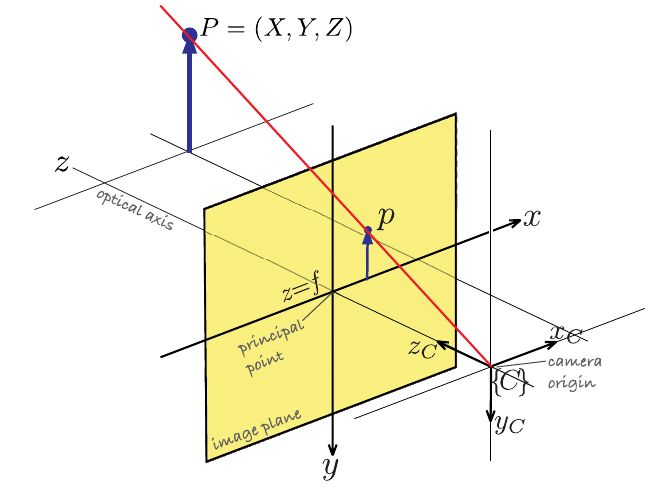
\includegraphics[width=.5\textwidth]{centralProjModel}
\end{figure}
\[
\left (
\begin{array}{c}
\tilde{x}\\
\tilde{y}\\
\tilde{z}
\end{array}
\right )
=
\left (
\begin{array}{cccc}
f & 0 & 0 & 0 \\
0 & f & 0 & 0 \\
0 & 0 & 1 & 0
\end{array}
\right )
\left (
\begin{array}{c}
X \\
Y \\
Z \\
1
\end{array}
\right )
\]
\end{frame}

\begin{frame}
\frametitle{Central Projection Model}
\begin{columns}
\begin{column}{.5\textwidth}
\begin{figure}[!h]
\centering
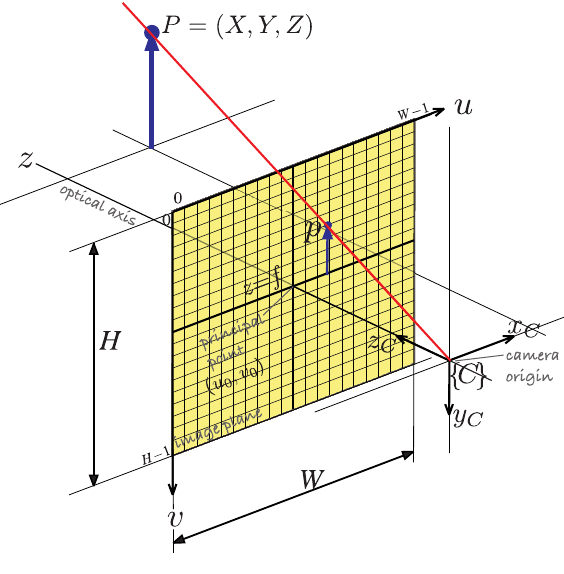
\includegraphics[width=\textwidth]{centralProjModel-2}
\end{figure}
\end{column}
\begin{column}{.5\textwidth}
\[
\left (
\begin{array}{c}
\tilde{u} \\
\tilde{v} \\
\tilde{w}
\end{array}
\right )
=
\left (
\begin{array}{ccc}
\dfrac{1}{\rho_u} & 0 & u_{0} \\
0 & \dfrac{1}{\rho_v} & v_{0} \\
0 & 0 & 1
\end{array}
\right )
\left (
\begin{array}{c}
\tilde{x}\\
\tilde{y}\\
\tilde{z}
\end{array}
\right )
\]
\begin{itemize}
\item Scale from meters to pixels.
\item Shift the origin to top left corner.
\end{itemize}
\[
p =
\left (
\begin{array}{c}
\tilde{u} \\
\tilde{v}
\end{array}
\right )
=
\left (
\begin{array}{c}
\tilde{u}/\tilde{w} \\
\tilde{v}/\tilde{w}
\end{array}
\right )
\]
\end{column}
\end{columns}
\end{frame}

\begin{frame}
\footnotesize
\begin{columns}
\begin{column}{.5\textwidth}
\begin{figure}[!h]
\centering
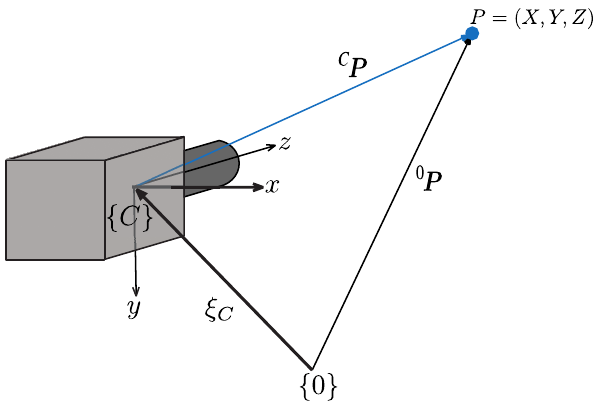
\includegraphics[width=\textwidth]{camera}
\end{figure}
\end{column}
\begin{column}{.5\textwidth}
\[
\left (
\begin{array}{c}
\tilde{x}\\
\tilde{y}\\
\tilde{z}
\end{array}
\right )
=
\left (
\begin{array}{cccc}
f & 0 & 0 & 0 \\
0 & f & 0 & 0 \\
0 & 0 & 1 & 0
\end{array}
\right )
\left (
\begin{array}{c}
X \\
Y \\
Z \\
1
\end{array}
\right )
\]
\end{column}
\end{columns}
\[
\boxed{
\left (
\begin{array}{c}
\tilde{u} \\
\tilde{v} \\
\tilde{w}
\end{array}
\right )
=
\underbrace{
\underbrace{
\left (
\begin{array}{ccc}
\dfrac{1}{\rho_u} & 0 & u_{0} \\
0 & \dfrac{1}{\rho_v} & v_{0} \\
0 & 0 & 1
\end{array}
\right )
\left (
\begin{array}{cccc}
f & 0 & 0 & 0 \\
0 & f & 0 & 0 \\
0 & 0 & 1 & 0
\end{array}
\right )
}_{K=\text{intrinsic parameters}}
\underbrace{
\left (
\begin{array}{cc}
\textbf{\text{R}} & t \\
\textbf{\text{0}}_{1\times 3} & 1
\end{array}
\right )^{-1}
}_{\text{extrinsic parameters}}
}_{C = \text{camera matrix}}
\left (
\begin{array}{c}
X \\
Y \\
Z \\
1
\end{array}
\right )
}
\]
\end{frame}

\begin{frame}
\footnotesize
\[
\boxed{
\left (
\begin{array}{c}
\tilde{u} \\
\tilde{v} \\
\tilde{w}
\end{array}
\right )
=
\underbrace{
\underbrace{
\left (
\begin{array}{ccc}
\dfrac{1}{\rho_u} & 0 & u_{0} \\
0 & \dfrac{1}{\rho_v} & v_{0} \\
0 & 0 & 1
\end{array}
\right )
\left (
\begin{array}{cccc}
f & 0 & 0 & 0 \\
0 & f & 0 & 0 \\
0 & 0 & 1 & 0
\end{array}
\right )
}_{K=\text{intrinsic parameters}}
\underbrace{
\left (
\begin{array}{cc}
\textbf{\text{R}} & t \\
\textbf{\text{0}}_{1\times 3} & 1
\end{array}
\right )^{-1}
}_{\text{extrinsic parameters}}
}_{C = \text{camera matrix}}
\left (
\begin{array}{c}
X \\
Y \\
Z \\
1
\end{array}
\right )
}
\]
\begin{itemize}
\item Intrinsic parameters (5): $f$, $\rho_u$, $\rho_v$, $u_0$ and $v_0$.
\item Extrinsic parameters (6): Rotation and translation.
\end{itemize}
\begin{block}{Camera parameters}
Initially unknown and estimated using a calibration procedure.
\end{block}
\end{frame}

\begin{frame}
\frametitle{Camera matrix}
\begin{itemize}
\item Mapping points from the world to an image (pixel) coordinate is simply a matrix multipliaction using
\end{itemize}
\[
\left (
\begin{array}{c}
\tilde{u} \\
\tilde{v} \\
\tilde{w}
\end{array}
\right )
=
\left (
\begin{array}{cccc}
C_{11} & C_{12} & C_{13} & C_{14} \\
C_{21} & C_{22} & C_{23} & C_{24} \\
C_{31} & C_{32} & C_{33} & C_{34} \\
\end{array}
\right )
\left (
\begin{array}{c}
X \\
Y \\
Z \\
1
\end{array}
\right )
\]
And:
\[
p =
\left (
\begin{array}{c}
\tilde{u} \\
\tilde{v}
\end{array}
\right )
=
\left (
\begin{array}{c}
\tilde{u}/\tilde{w} \\
\tilde{v}/\tilde{w}
\end{array}
\right )
\]
\end{frame}

\section{Field of View (FOV)}

\begin{frame}
\frametitle{Field of View (FOV)}
\begin{itemize}
\item The field of view of a lens is an open rectangular pyramid that subtends angles $\theta_h$ and $\theta_v$ in the horizontal and vertical planes respectively.
\item The dimension of a sensor chip $d$ is measured diagonally between its corners and is typically expressed in inches.
\item Common dimensions are $1/4$, $1/3$ and $1/2$ inch.
\item A normal lens has $f \approx d$ and a wide-angle lens generally has $f > d/3$ giving a maximum angular field of view of $\approx 110 ^{\circ}$.
\end{itemize}
\end{frame}

\begin{frame}
\frametitle{Field of View (FOV)}
\begin{itemize}
\item For wide-angle lenses it is more common to describe the field of view as a solid angle which is measured in units of steradians (or sr).
\item This is the area of the field of view projected onto the surface of a unit sphere.
\item A hemispherical field of view is $2\pi$~sr and a full spherical view is $4\pi$~sr.
\item If we approximate the camera's field of view by a cone with apex angle $\theta$ the corresponding solid angle is $\Omega = 2\pi(1-cos\theta/2)$~sr.
\item A camera with a field of view greater than a full hemisphere is termed omni-directional or panoramic.
\end{itemize}
\end{frame}

\begin{frame}
\frametitle{Field of View (FOV)}
\begin{itemize}
\item The field of view of a camera is a function of its focal length $f$.
\item A wide-angle lens has a small focal length.
\item A telephoto lens has a large focal length
\item A zoom lens has an adjustable focal length. 
\end{itemize}
\end{frame}

\begin{frame}
\frametitle{Field of View (FOV)}
\begin{columns}
\begin{column}{.5\textwidth}
\begin{figure}[!h]
\centering
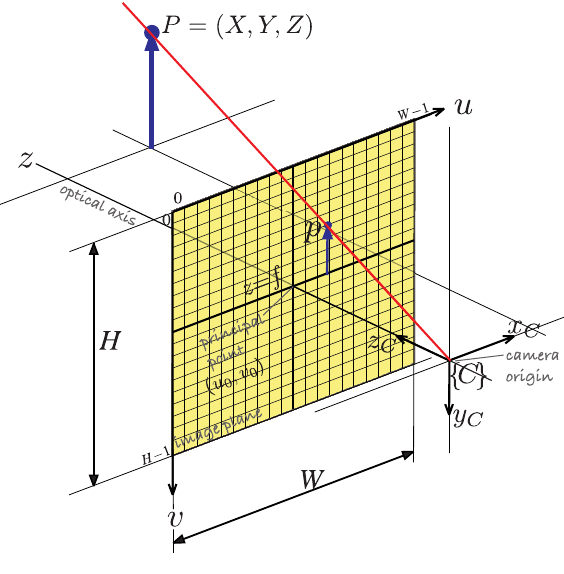
\includegraphics[width=\textwidth]{centralProjModel-2}
\end{figure}
\end{column}
\begin{column}{.5\textwidth}
\begin{itemize}
\item Horizontal angle view:
\[
\theta_{h} = 2 \tan^{-1} \dfrac{\rho_u W/2}{f}
\]
\item Vertical angle view:
\[
\theta_{v} = 2 \tan^{-1} \dfrac{\rho_v H/2}{f}
\]
\item Note that the FOV depends on the dimensions of the camera chip, ie., $W\rho^{u} \times H\rho_{v}$.
\end{itemize}
\end{column}
\end{columns}
\end{frame}



\begin{frame}[fragile]
\frametitle{Camera matrix}
Given the following camera matrix
\begin{lstlisting}
C = [...
    512     -800    0       800; ...
    512     0       -800    1600; ...
    1       0       0       0
    ];
\end{lstlisting}
Find the image coordinates of point $P = \left ( \begin{array}{ccc}
4 & 0 & 0 
\end{array}
\right )^{T}$
\end{frame}


\begin{frame}[fragile]
\frametitle{Camera matrix}
\begin{lstlisting}
C = [...
    512     -800    0       800; ...
    512     0       -800    1600; ...
    1       0       0       0
    ];
P = [4, 0, 0];
W = C * [P, 1]'
W = W/W(3)
\end{lstlisting}
\end{frame}

\begin{frame}
\frametitle{Scale invariance}
\begin{itemize}
\item Consider an arbitrary scalar scale factor
\[
\left (
\begin{array}{c}
\tilde{u} \\
\tilde{v} \\
\tilde{w}
\end{array}
\right )
=
\lambda
\left (
\begin{array}{cccc}
C_{11} & C_{12} & C_{13} & C_{14} \\
C_{21} & C_{22} & C_{23} & C_{24} \\
C_{31} & C_{32} & C_{33} & C_{34} \\
\end{array}
\right )
\left (
\begin{array}{c}
X \\
Y \\
Z \\
1
\end{array}
\right )
\]
\item $\tilde{u}, \tilde{v}, \tilde{w}$ will all be scaled by $\lambda$.
\item but
\[
u=\dfrac{\tilde{u}}{\tilde{w}},\ v = \dfrac{\tilde{v}}{\tilde{w}}.
\]
\item So the result is unchanged.
\end{itemize}
\end{frame}

\begin{frame}
\frametitle{Normalized camera matrix}
Since scale factor is arbitrary we can fix the value of one element, typically $C(3,4)$ to one.
\[
\left (
\begin{array}{c}
\tilde{u} \\
\tilde{v} \\
\tilde{w}
\end{array}
\right )
=
\lambda
\left (
\begin{array}{cccc}
C_{11} & C_{12} & C_{13} & C_{14} \\
C_{21} & C_{22} & C_{23} & C_{24} \\
C_{31} & C_{32} & C_{33} & 1 \\
\end{array}
\right )
\left (
\begin{array}{c}
X \\
Y \\
Z \\
1
\end{array}
\right )
\]
\end{frame}

\begin{frame}[fragile]
\frametitle{Example}
\begin{lstlisting}
cam = CentralCamera('default', 'pose', ...
    transl(0,1,2)*troty(pi/2)*trotz(-pi/2));
cam.C
P = [4,0,0]';
cam.project(P)
\end{lstlisting}
\end{frame}

\begin{frame}[fragile]
Example
\begin{columns}
\begin{column}{.5\textwidth}
\begin{lstlisting}[language=Matlab]
%%
cam = CentralCamera(...
	'default', 'pose', ...
    transl(0,1,2)*...
    troty(pi/2)*...
    \\
    trotz(-pi/2));
cam.C
P = [4,0,0]';
cam.project(P)
cam.plot_camera
plot_sphere(P, 0.05)
grid on
\end{lstlisting}
\end{column}
\begin{column}{.5\textwidth}
\begin{figure}[!h]
\centering
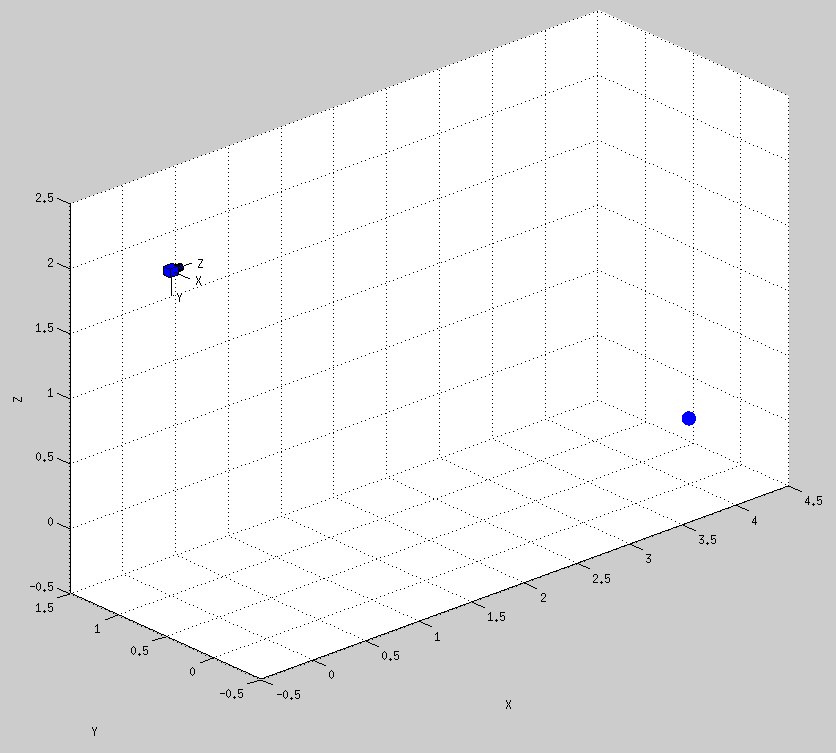
\includegraphics[width=\textwidth]{cam-plot}
\end{figure}
\end{column}
\end{columns}
\end{frame}

\begin{frame}[fragile]
\frametitle{Camera matrix}
Find the camera's matrices:
\begin{lstlisting}[language=Matlab]
cam.C
cam.K
cam.fov() * 180/pi
\end{lstlisting}
\end{frame}

\begin{frame}[fragile]
Example
\begin{lstlisting}
cam = CentralCamera('focal', 0.015, ...
    'pixel', 10e-6, ... 
    'resolution', [1280 1024], ...
    'centre', [640 512], 'name', 'mycamera')
P = mkgrid(3, 0.2, 'T', transl(0, 0, 1.0));
cam.project(P)
cam.plot(P)
\end{lstlisting}
\begin{figure}[!h]
\centering
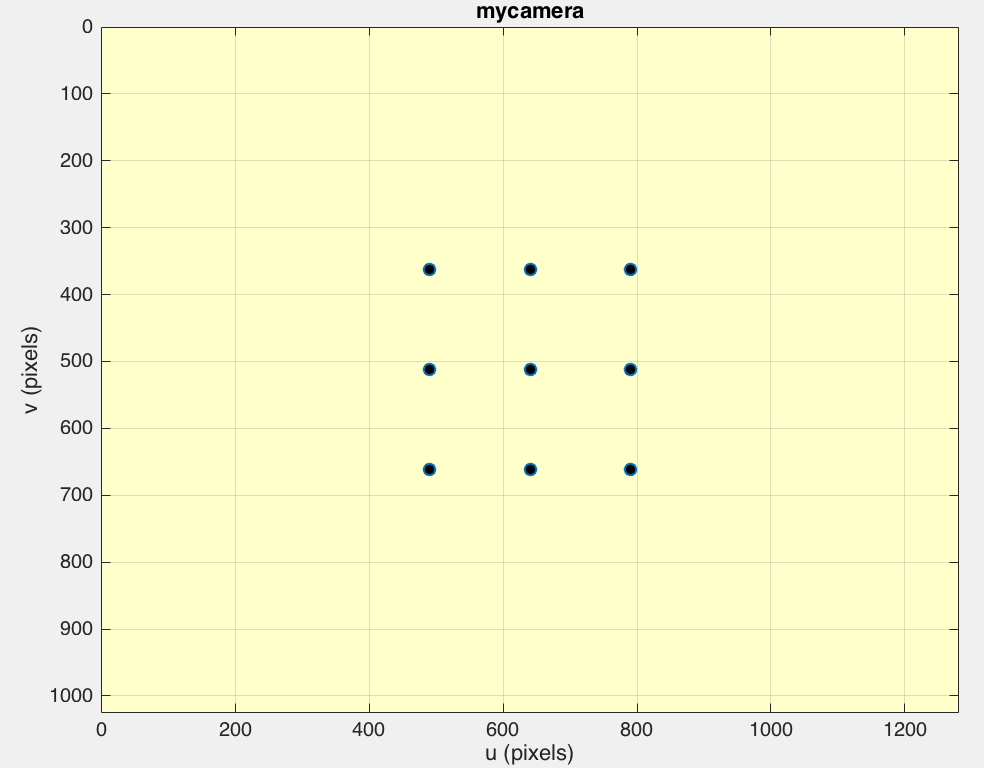
\includegraphics[width=.3\textwidth]{gridTarget}
\end{figure}
\end{frame}

\begin{frame}[fragile]
Example
\begin{lstlisting}
Tcam = transl(-1,0,0.5)*troty(0.9);
cam.plot(P, 'Tcam', Tcam)
\end{lstlisting}
\begin{figure}[!h]
\centering
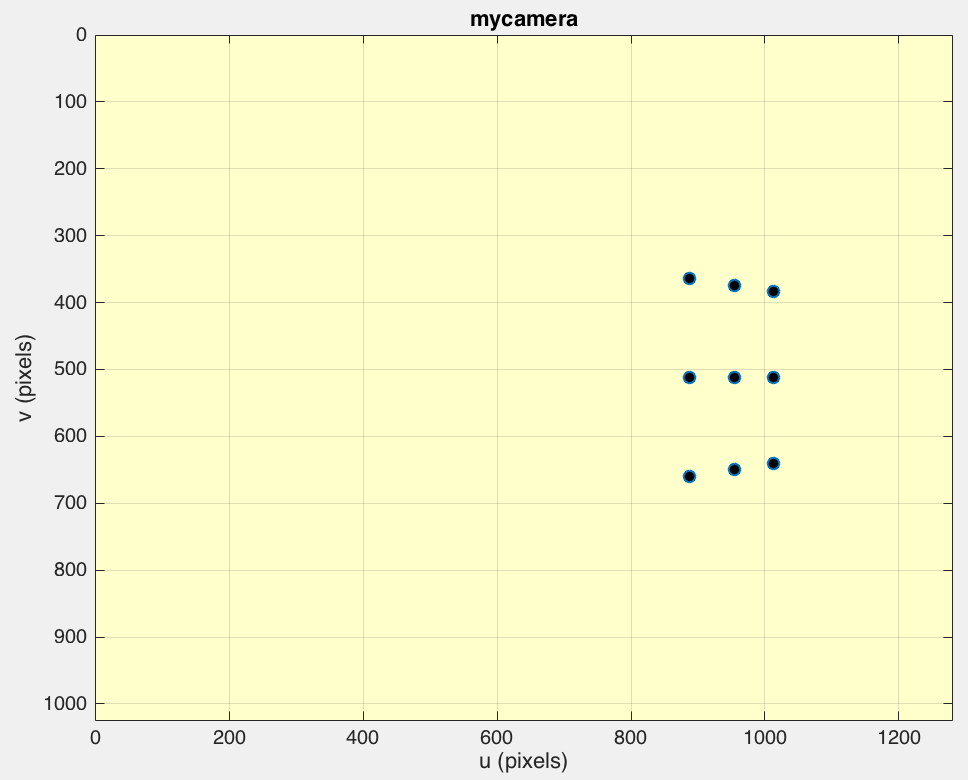
\includegraphics[width=.4\textwidth]{gridTarget2}
\end{figure}
\end{frame}

\begin{frame}[fragile]
\begin{lstlisting}
cam = CentralCamera('focal', 0.015, ...
    'pixel', 10e-6, ... 
    'resolution', [1280 1024], ...
    'centre', [640 512], 'name', 'mycamera')
cube = mkcube(0.2, 'T', transl([0, 0, 1]) );
[X,Y,Z] = mkcube(0.2, 'T', transl([0, 0, 1.0]), 'edge');
cam.mesh(X, Y, Z)
\end{lstlisting}
\begin{figure}[!h]
\centering
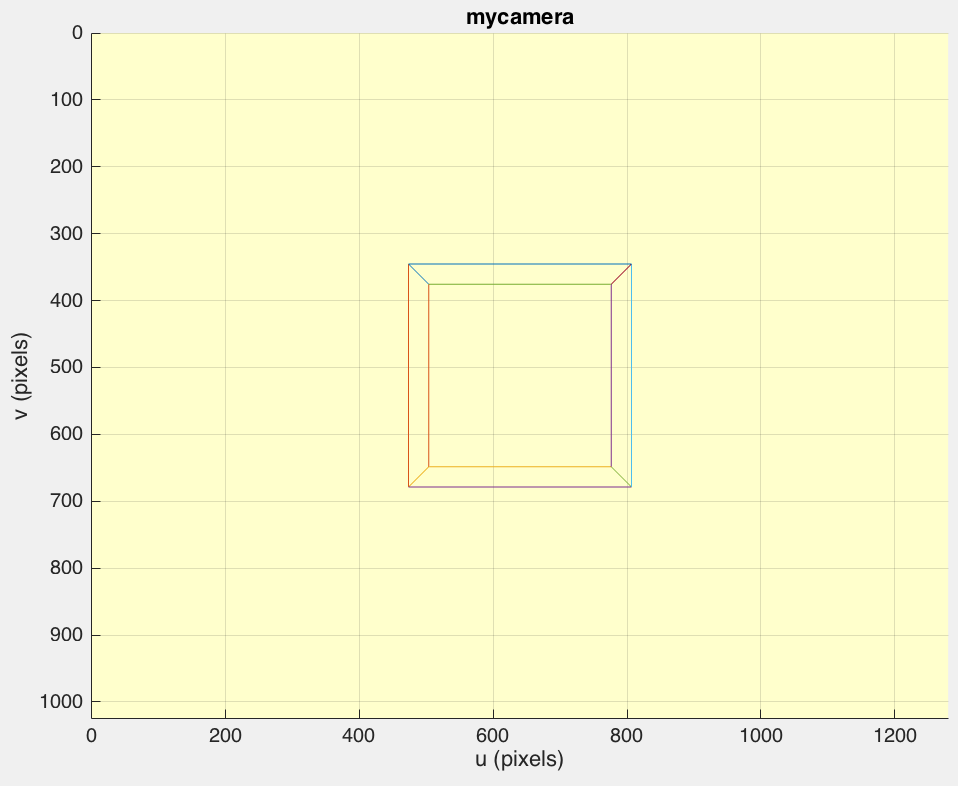
\includegraphics[width=.3\textwidth]{cube}
\end{figure}
\end{frame}

\begin{frame}[fragile]
\begin{lstlisting}
cam = CentralCamera('focal', 0.015, ...
    'pixel', 10e-6, ... 
    'resolution', [1280 1024], ...
    'centre', [640 512], 'name', 'mycamera')
cube = mkcube(0.2, 'T', transl([0, 0, 1]) );
[X,Y,Z] = mkcube(0.2, 'T', transl([0, 0, 1.0]), 'edge');
cam.T = transl(-1,0,0.5)*troty(0.8);
cam.mesh(X, Y, Z, 'Tcam', Tcam);
\end{lstlisting}
\begin{figure}[!h]
\centering
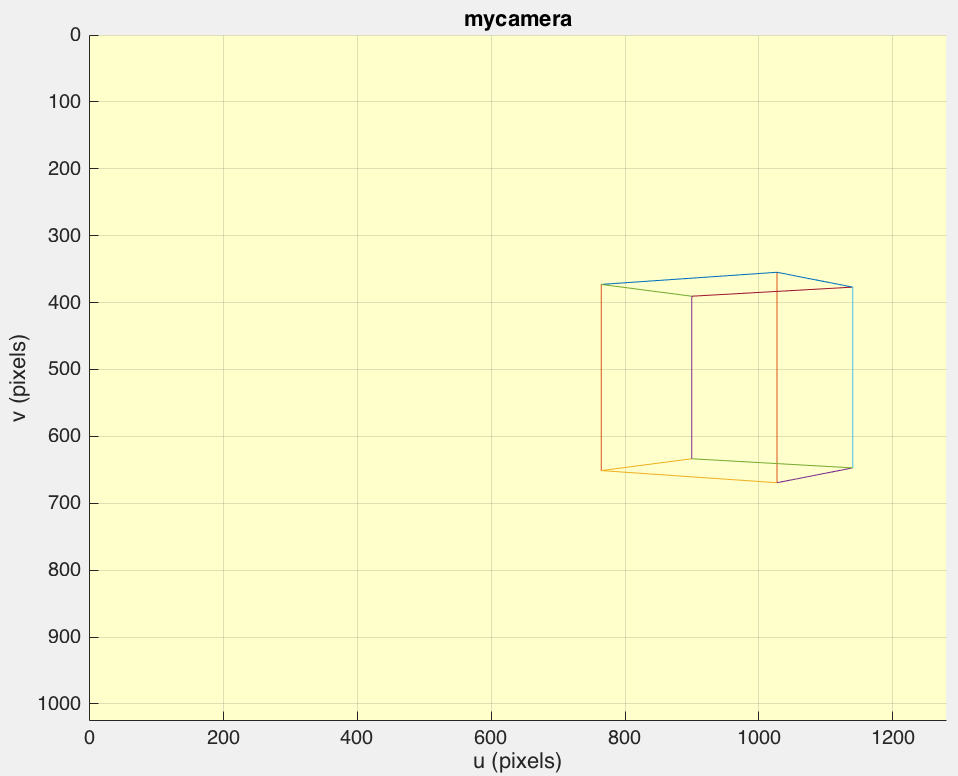
\includegraphics[width=.3\textwidth]{cube2}
\end{figure}
\end{frame}

\begin{frame}[fragile]
\begin{lstlisting}
cam = CentralCamera('focal', 0.015, ...
    'pixel', 10e-6, ... 
    'resolution', [1280 1024], ...
    'centre', [640 512], 'name', 'mycamera')
theta = [0:20]/100*2*pi;
[X,Y,Z] = mkcube(0.2, [], 'edge');
for th = theta
    T_cube = transl(0, 0, 1.5)*trotx(th)*...
    	troty(th*1.2)*trotz(th*1.3)
    [X,Y,Z] = mkcube(0.2, 'T', T_cube, 'edge');
    cam.mesh(X, Y, Z, 'Tcam', Tcam);
    pause(.01);
end
\end{lstlisting}
\end{frame}

\section{Planar homography}

\begin{frame}
\frametitle{Planar homography}
\begin{figure}[!h]
\centering
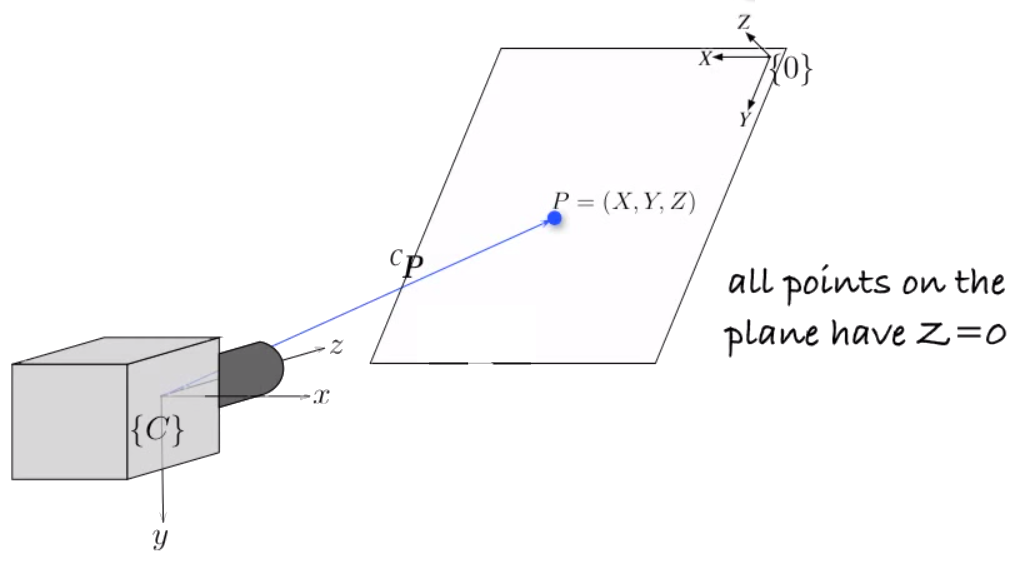
\includegraphics[width=.6\textwidth]{plane}
\end{figure}
\[
\left (
\begin{array}{c}
\tilde{u} \\
\tilde{v} \\
\tilde{w}
\end{array}
\right )
=
\left (
\begin{array}{cccc}
C_{11} & C_{12} & C_{13} & C_{14} \\
C_{21} & C_{22} & C_{23} & C_{24} \\
C_{31} & C_{32} & C_{33} & 1 \\
\end{array}
\right )
\left (
\begin{array}{c}
X \\
Y \\
0 \\
1
\end{array}
\right )
\]
\end{frame}

\begin{frame}
\frametitle{Planar homography}
\[
\left (
\begin{array}{c}
\tilde{u} \\
\tilde{v} \\
\tilde{w}
\end{array}
\right )
=
\left (
\begin{array}{ccc}
H_{11} & H_{12} & H_{13} \\
H_{21} & H_{22} & H_{23} \\
H_{31} & H_{32} & 1 \\
\end{array}
\right )
\left (
\begin{array}{c}
X \\
Y \\
1
\end{array}
\right )
\]
\begin{itemize}
\item Once again the scale factor is arbitrary.
\item 8 unique numbers in the homography matrix.
\item Can be estimated from 4 world points and their corresponding image points.
\end{itemize}
\end{frame}

\begin{frame}
\frametitle{Perspective rectification}
\begin{figure}[!h]
\centering
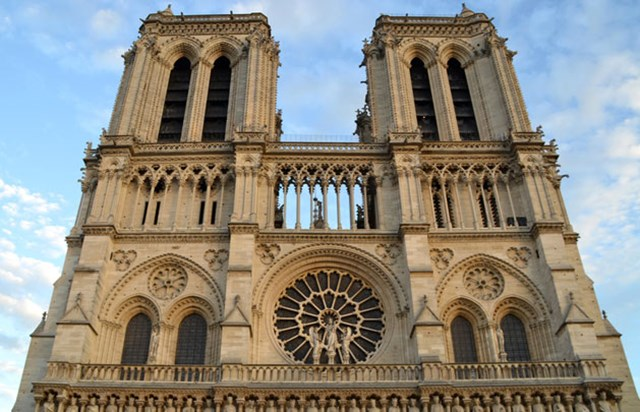
\includegraphics[width=.6\textwidth]{notreDame}
\end{figure}
\end{frame}

\begin{frame}[fragile]
\frametitle{Perspective rectification}
\begin{figure}[!h]
\centering
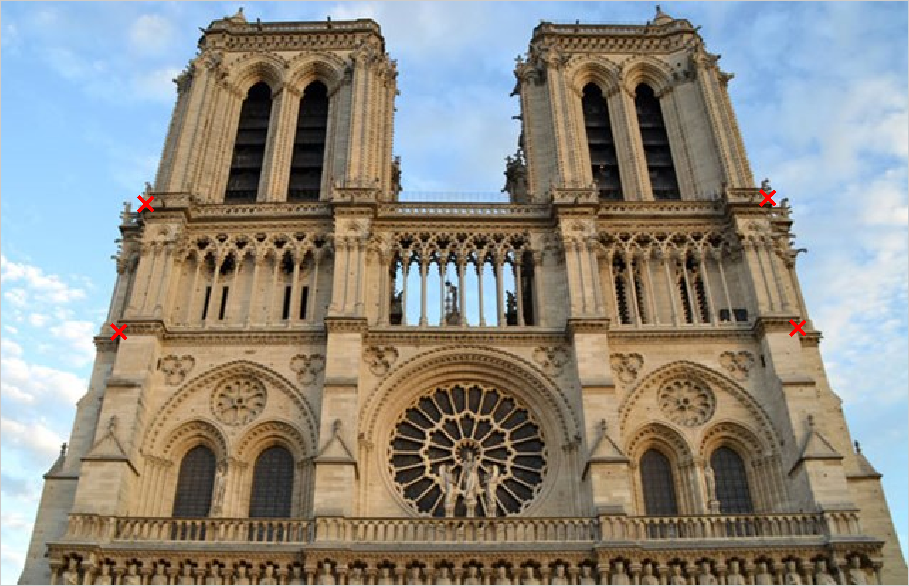
\includegraphics[width=.6\textwidth]{notreDame1}
\end{figure}
\begin{lstlisting}
[x, y] = ginput(4)
\end{lstlisting}
\end{frame}

\begin{frame}[fragile]
\frametitle{Perspective rectification}
\begin{figure}[!h]
\centering
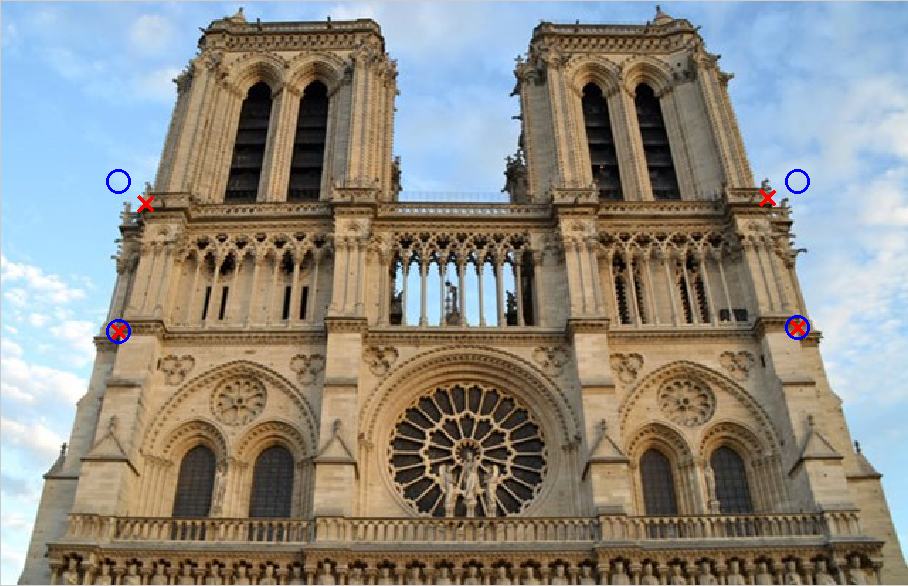
\includegraphics[width=.6\textwidth]{notreDame2}
\end{figure}
\begin{lstlisting}
H = homography([x, y]', [x2, y2]')
\end{lstlisting}
\[
^{2}p = \textbf{\text{H}} ^{1}p
\]
\end{frame}

\begin{frame}[fragile]
\frametitle{Perspective rectification}
\begin{figure}[!h]
\centering
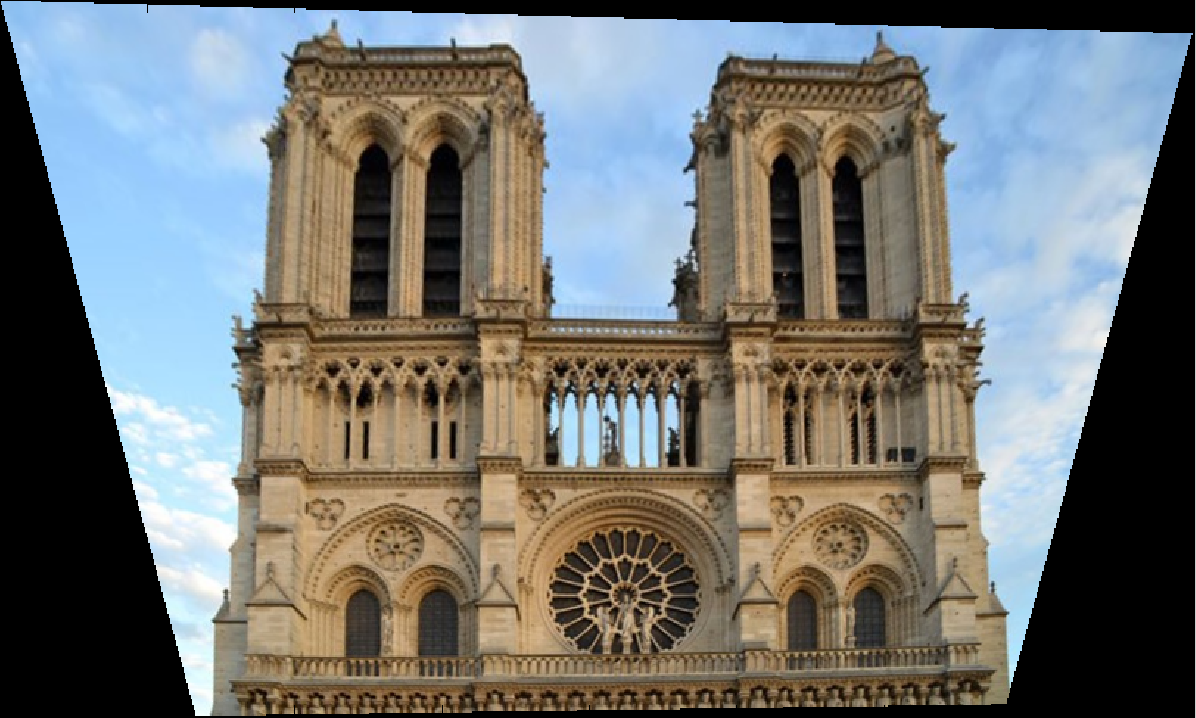
\includegraphics[width=.6\textwidth]{notreDame3}
\end{figure}
\begin{lstlisting}
homwarp(H, f, 'full')
\end{lstlisting}
\end{frame}

\begin{frame}
\frametitle{Virtual camera}
\begin{figure}[!h]
\centering
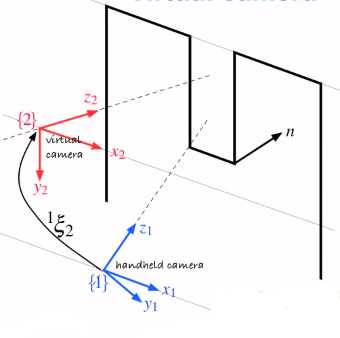
\includegraphics[width=.5\textwidth]{virtualCam}
\end{figure}
\[
H_{E} \approx R + \dfrac{t}{d} n^{T}
\]
\end{frame}

\begin{frame}
\begin{figure}[!h]
\centering
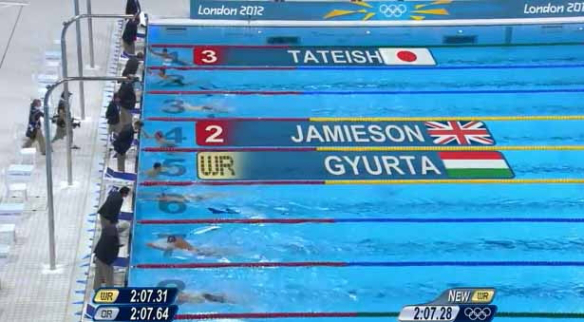
\includegraphics[width=\textwidth]{olympicPool}
\end{figure}
\end{frame}

\section{Lens distortion}

\begin{frame}
\frametitle{Lens distortion}
No lenses are perfect:
\begin{itemize}
\item Chromatic aberration (color fringing).
\item Spherical aberration astigmatism (variation in focus accross the scene).
\end{itemize}
\begin{block}{Geometric distortion}
Most problematic effect in computer vision.\\
Two components:
\begin{enumerate}
\item Radial.
\item Tangential.
\end{enumerate}
\end{block}
\end{frame}

\begin{frame}
\frametitle{Lens distortion}
Tangential distortion. Displacement between the lens principal axis and the sensor's geometric center.\\
\end{frame}

\begin{frame}
\frametitle{Lens distortion}
\begin{columns}
\begin{column}{.5\textwidth}
The radial error is approximated by
\begin{equation}
\delta r = k_{1} r^{3} + k_{2} r^{5} + k_{3} r^{7} + \ldots
\end{equation}
where $r$ is the distance from the image point to the sensor's principal point.
\end{column}
\begin{column}{.5\textwidth}
\begin{figure}[!h]
\centering
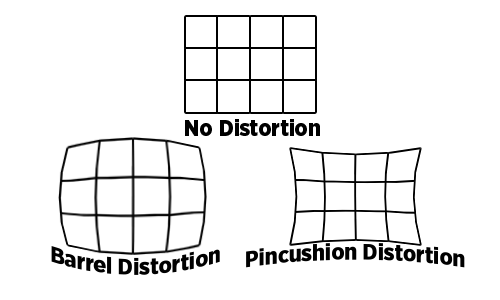
\includegraphics[width=\textwidth]{radialDistortion}
\end{figure}
\end{column}
\end{columns}
\end{frame}

\begin{frame}
\frametitle{Lens distortion}
The coordinates $(u,v)$ of a point, after distortion are given by
\begin{equation}
\begin{array}{c}
u^{(d)} = u + \delta_u \\
v^{(d)} = v + \delta	_v
\end{array}
\end{equation}
Where the displacement is
\footnotesize
\begin{equation}
\left (
\begin{array}{c}
\delta_u \\
\delta_v
\end{array}
\right )
=
\underbrace{
\left (
\begin{array}{c}
u \left ( k_{1} r^{2} + k_{2} r^{4} + k_{3} r^{6} + \ldots \right ) \\
v \left ( k_{1} r^{2} + k_{2} r^{4} + k_{3} r^{6} + \ldots \right )
\end{array}
\right )
}_{\text{radial}}
+
\underbrace{
\left (
\begin{array}{c}
2p_{1} uv + p_{2} (r^{2} + 2 u^{2})\\
p_1 ( r^{2} + 2v^{2} ) + 2p_1 uv
\end{array}
\right )
}_{\text{tangential}}
\end{equation}
\end{frame}

\begin{frame}
\frametitle{Lens distortion}
\begin{figure}[!h]
\centering
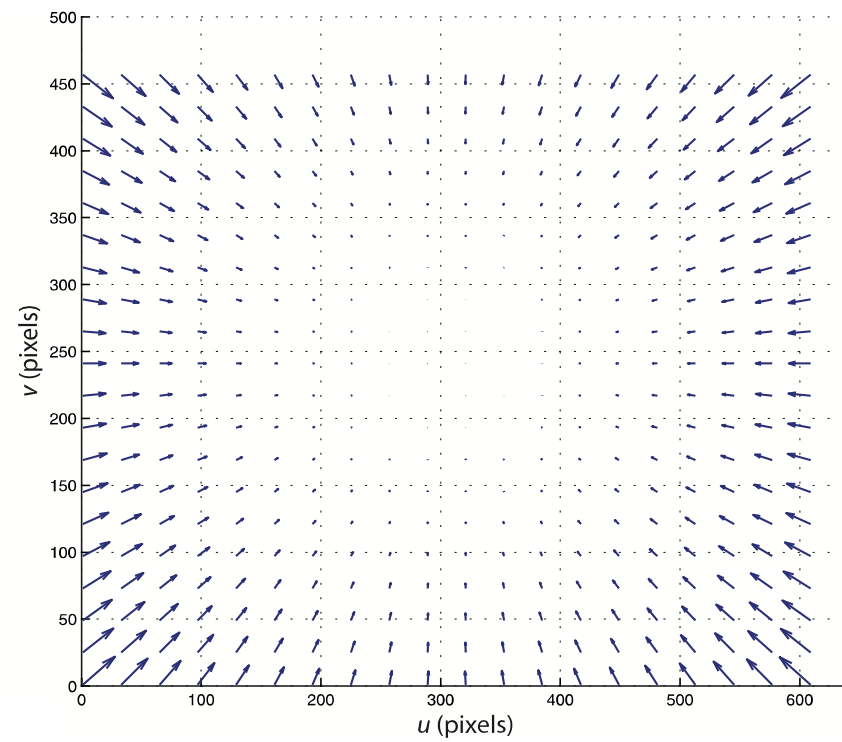
\includegraphics[width=.6\textwidth]{displacementVectorField}
\end{figure}
\end{frame}

\begin{frame}[fragile]
Typically three coefficients are sufficient to describe the radial distortion and the distortion model is parameterized by (k1, k2, k3, p1, p2) which are considered as additional intrinsic parameters. Distortion can be modeled by the CentralCamera class using the 'distortion' option, for example
\begin{lstlisting}
cam = CentralCamera('focal', 0.015, ...
    'pixel', 10e-6, ... 
    'resolution', [1280 1024], ...
    'centre', [512 512], ... 
    'distortion', [k1 k2 k3 p1 p2] )
\end{lstlisting}
\end{frame}

\section{Camera calibration}

\subsection{Homogeneous Transformation Approach}

\begin{frame}[fragile]
\frametitle{Camera calibration}
A linear calibration model (book).\\
Example:
\begin{lstlisting}
P = mkcube(0.2);
T_unknown = transl(0.1, 0.2, 1.5) * ...
    rpy2tr(0.1, 0.2, 0.3);
cam = CentralCamera('focal', 0.015, ...
    'pixel', 10e-6, ...
    'resolution', [1280 1024], ...
    'centre', [512 512], ... 
    'noise', 0.05);
p = cam.project(P, 'Tobj', T_unknown);
C = camcald(P, p)
\end{lstlisting}
\end{frame}

\subsection{Decomposing the Camera Calibration Matrix}

\begin{frame}[fragile]
\begin{lstlisting}
% Decomposing the Camera Calibration Matrix
est = invcamcal(C) % Attention! invcamcal_updated
est.f/est.rho(1)
cam.f/cam.rho(2)

T_unknown * est.T

est.plot_camera()
\end{lstlisting}
\end{frame}

\subsection{Post estimation}

\begin{frame}[fragile]
\frametitle{Pose Estimation}
\begin{lstlisting}
cam = CentralCamera('focal', 0.015, ...
    'pixel', 10e-6, ... 
    'resolution', [1280 1024], ...
    'centre', [640 512]);
P = mkcube(0.2);
T_unknown = transl(0,0,2)*trotx(0.1)*troty(0.2)
p = cam.project(P, 'Tobj', T_unknown);
T_est = cam.estpose(P, p)
\end{lstlisting}
\end{frame}

\begin{frame}[fragile]
\frametitle{Pose Estimation}
\begin{lstlisting}
T_unknown =

    0.9801         0    0.1987         0
    0.0198    0.9950   -0.0978         0
   -0.1977    0.0998    0.9752    2.0000
         0         0         0    1.0000


T_est =

    0.9801    0.0000    0.1987   -0.0000
    0.0198    0.9950   -0.0978    0.0000
   -0.1977    0.0998    0.9752    2.0000
         0         0         0    1.0000
\end{lstlisting}
\end{frame}

\begin{frame}[fragile]
\frametitle{Pose Estimation}
\begin{lstlisting}
cam = CentralCamera('focal', 0.015, ...
    'pixel', 10e-6, ... 
    'resolution', [1280 1024], ...
    'centre', [640 512], ... 
    'noise', 0.05);
P = mkcube(0.2);
T_unknown = transl(0,0,2)*trotx(0.1)*troty(0.2)
p = cam.project(P, 'Tobj', T_unknown);
T_est = cam.estpose(P, p)
\end{lstlisting}
\end{frame}

\begin{frame}[fragile]
\begin{lstlisting}
T_unknown =

    0.9801         0    0.1987         0
    0.0198    0.9950   -0.0978         0
   -0.1977    0.0998    0.9752    2.0000
         0         0         0    1.0000


T_est =

    0.9794    0.0002    0.2020   -0.0001
    0.0204    0.9948   -0.0999    0.0000
   -0.2009    0.1019    0.9743    2.0019
         0         0         0    1.0000
\end{lstlisting}
\end{frame}

\subsection{Camera Calibration Toolbox}

\begin{frame}[fragile]
\frametitle{Camera Calibration Toolbox}
\begin{itemize}
\item Camera Calibration Toolbox for Matlab \url{https://www.vision.caltech.edu/bouguetj/calib_doc/}
\begin{lstlisting}
calib_gui
\end{lstlisting}
\item Camera calibration APP (Matlab).
\item Stereo camera calibration APP (Matlab).
\end{itemize}
\end{frame}

\section{Non-Perspective Imaging Models}

\begin{frame}
Non-Perspective Imaging Models
\begin{columns}
\begin{column}{.5\textwidth}
\begin{itemize}
\item Perspective camera model mimics the way human-eye works.
\item FOV limited to one hemisfere.
\item Radial distortion increasingly higher for smaller focal length $f$.
\item Let's drop the perspective contrain and use reflection rather than refraction.
\item Mirrors are free of color fringing.
\item Easier to scale.
\end{itemize}
\end{column}
\begin{column}{.5\textwidth}
\begin{figure}[!h]
\centering
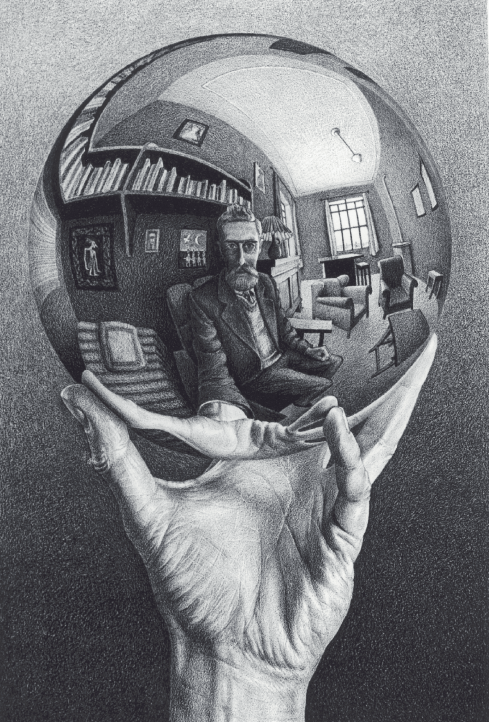
\includegraphics[width=.7\textwidth]{escher-sphere}
\caption{Escher (1935).}
\end{figure}
\end{column}
\end{columns}
\end{frame}

\subsection{Fisheye Lens Camera}

\begin{frame}
\frametitle{Fisheye Lens Camera}
\begin{columns}
\begin{column}{.7\textwidth}
\begin{figure}[!h]
\centering
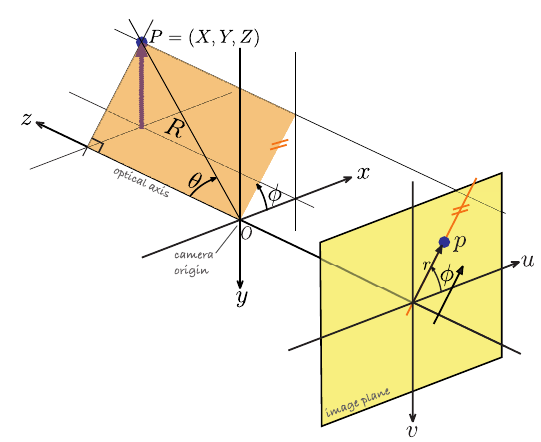
\includegraphics[width=\textwidth]{fisheye-model}
\end{figure}
\end{column}
\begin{column}{.4\textwidth}
\[
R = \sqrt{X^2 + Y^2 + Z^2}
\]
\[
\theta = \cos ^{-1} \dfrac{R}{Z}
\]
\[
\phi = \tan^{-1} \dfrac{Y}{X}
\]
\[
u = r\cos\phi
\]
\[
v = r\sin\phi
\]
\end{column}
\end{columns}
\end{frame}

\begin{frame}
\begin{figure}[!h]
\centering
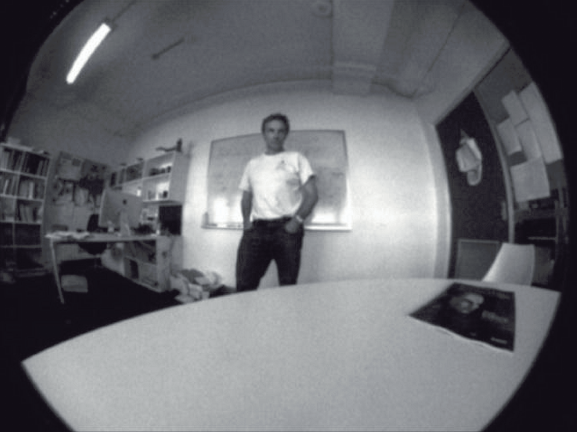
\includegraphics[width=.5\textwidth]{fisheye-lens-image}
\end{figure}
\begin{figure}[!h]
\centering
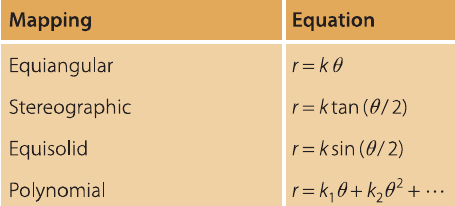
\includegraphics[width=.5\textwidth]{fisheye-proj-models}
\end{figure}
\end{frame}

\begin{frame}[fragile]
\begin{lstlisting}
cam = FishEyeCamera('name', 'fisheye', ...
    'projection', 'equiangular', ...
    'pixel', 10e-6, ...
    'resolution', [1280 1024])

[X,Y,Z] = mkcube(0.2, 'centre', [0.2, 0, 0.3], 'edge');
cam.mesh(X, Y, Z)
\end{lstlisting}
\end{frame}

\begin{frame}
Wide-angle lenses:
\begin{itemize}
\item Can have 180$^{\circ}$ or 190$^{\circ}$ FOV.
\item Spatial resolution is lower since the camera pixels are spread over a wider FOV.
\item The FOV is a circular region, i.e., nearly 25\% of the rectangular image plane is effectively wasted.
\item Outdoor images may reduce too much the exposure to avoid saturation.
\end{itemize}
\end{frame}

\subsection{Catadioptric Camera}

\begin{frame}
\frametitle{Catadioptric Camera}
\begin{block}{Catadioptric}
A catadioptric imaging system comprises both reflective and refractive elements, a mirror
and a lens
\end{block}
\begin{figure}[!h]
\centering
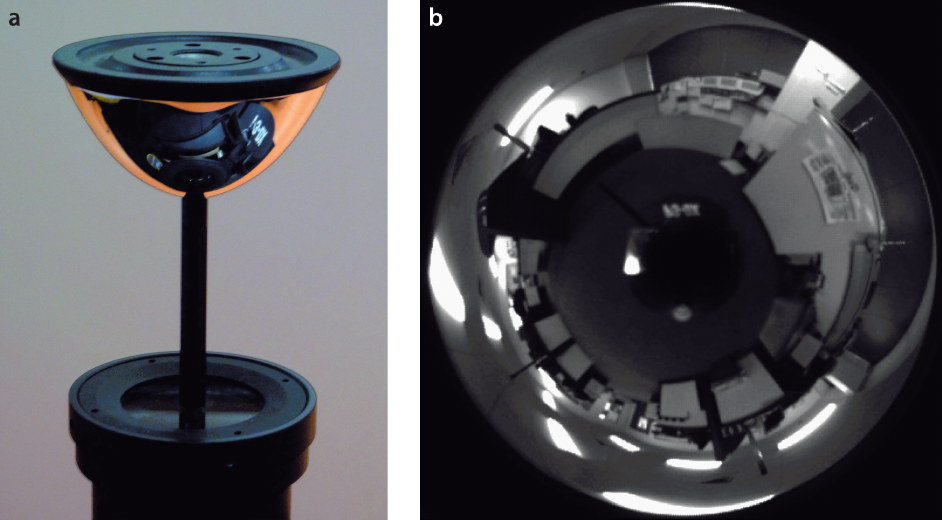
\includegraphics[width=.7\textwidth]{catadioptric}
\end{figure}
\end{frame}

%\begin{frame}
%\begin{figure}[!h]
%\centering
%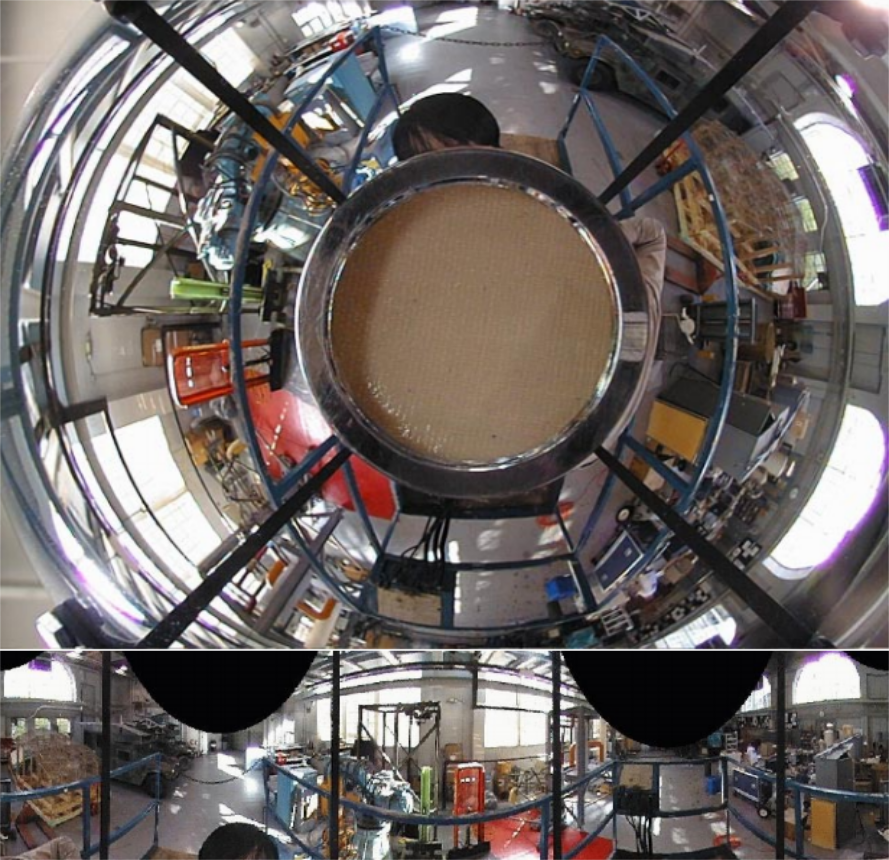
\includegraphics[width=.7\textwidth]{cm}
%\end{figure}
%\end{frame}

\begin{frame}
\begin{columns}
\begin{column}{.6\textwidth}
\begin{figure}[!h]
\centering
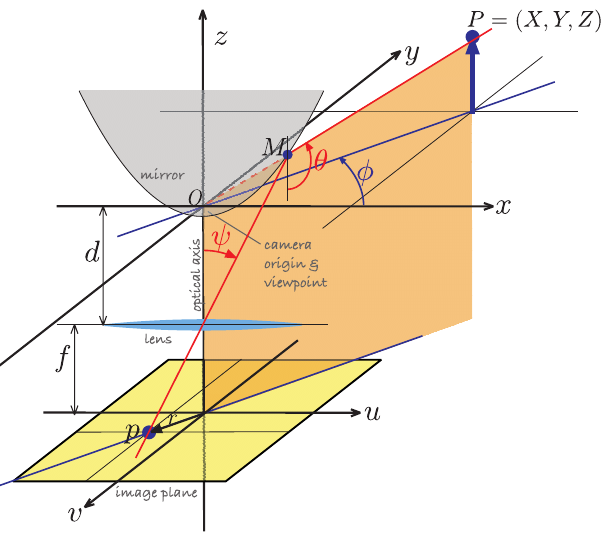
\includegraphics[width=1.1\textwidth]{catadioptric-cam-model}
\caption{Catadioptric image formation}
\end{figure}
\end{column}
\begin{column}{.4\textwidth}
\begin{itemize}
\item Elevation angle:
\[
\theta = \tan^{-1} \dfrac{Z}{X^{2} + Y^{2}} + \dfrac{\pi}{2}
\]
\[
a
\]
\item Relation between $\psi$ and $\theta$ is determined by the mirror shape at $M$.
\begin{itemize}
\item Spherical, parabolic, elliptical and hyperbolic.
\end{itemize}
\end{itemize}
\end{column}
\end{columns}
\end{frame}

\begin{frame}
\begin{block}{Equiangular mirror}
Each pixel spans an equal angle, irrespective of its distance from the center of the image.
\end{block}
\end{frame}

\begin{frame}
\begin{columns}
\begin{column}{.6\textwidth}
\begin{figure}[!h]
\centering
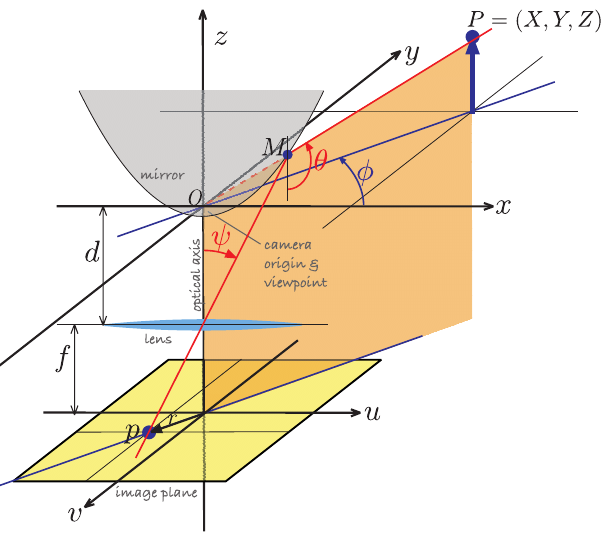
\includegraphics[width=\textwidth]{catadioptric-cam-model}
\caption{Catadioptric image formation}
\end{figure}
\end{column}
\begin{column}{.4\textwidth}
For equiangular mirrors, we have
\[
\theta = \alpha \psi
\]
\[
r = f \tan \psi
\]
\[
\textbf{p} = (r,\phi)
\]
\[
u = r\cos \phi
\]
\[
v = r\sin \phi
\]
where
\[
\phi = \tan^{-1} (Y/X)
\]
\end{column}
\end{columns}
\end{frame}

\begin{frame}[fragile]
\begin{lstlisting}
cam = CatadioptricCamera(...
    'name', 'panocam', ...
    'projection', 'equiangular', ...
    'maxangle', pi/4, ...
    'pixel', 10e-6, ...
    'resolution', [1280 1024])
[X,Y,Z] = mkcube(1, ...
    'centre', [1, 1, 0.8], 'edge');
cam.mesh(X, Y, Z)
\end{lstlisting}
\end{frame}

\begin{frame}
Advantages of catadioptric cameras:
\begin{itemize}
\item Can view 360$^\circ$ in azimuth.
\end{itemize}
Disadvantages of catadioptric cameras:
\begin{itemize}
\item Reduced spatial resolution.
\item Wasted image plane pixels.
\item Exposure control.
\item Blindspot.
\end{itemize}
\end{frame}

\subsection{Spherical camera}

\begin{frame}
\frametitle{Sherical camera}
\begin{figure}[!h]
\centering
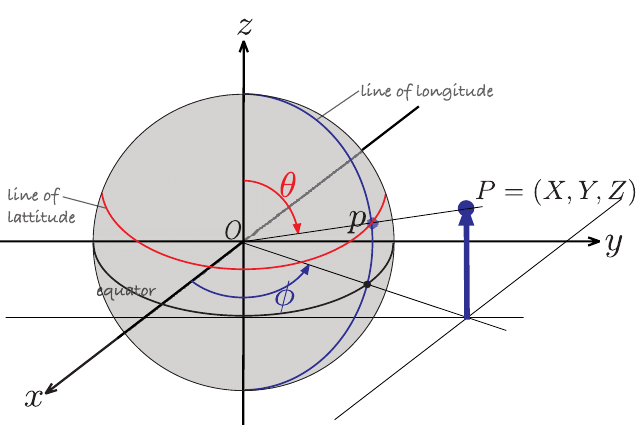
\includegraphics[width=.8\textwidth]{spherical-im-formation}
\end{figure}
\end{frame}

\begin{frame}
\frametitle{Sherical camera}
\begin{columns}
\begin{column}{.5\textwidth}
\begin{figure}[!h]
\centering
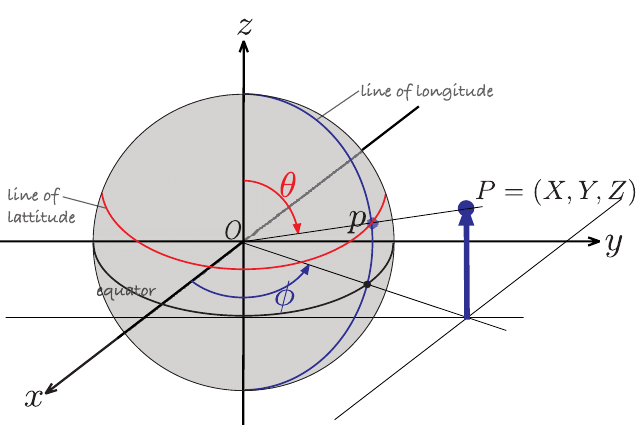
\includegraphics[width=\textwidth]{spherical-im-formation}
\end{figure}
\end{column}
\begin{column}{.5\textwidth}
\[
x=\dfrac{X}{R},\ y=\dfrac{Y}{R},\ z=\dfrac{Z}{R}
\]
\[
R = \sqrt{X^2 + Y^2 + Z^2}
\]
\[
\theta = \sin ^{-1} r,\ \theta \in  [0,\pi]
\]
\[
r = \sqrt{x^2 + y^2}
\]
\[
\phi = \tan ^{-1} \dfrac{y}{x},\ \phi \in [-\pi, \pi)
\]
\[
x = r\cos \phi
\]
\[
y = r\sin \phi
\]
\[
z = \cos \theta
\]
\end{column}
\end{columns}
\end{frame}

\begin{frame}[fragile]
\frametitle{Sherical camera}
\begin{lstlisting}
cam = SphericalCamera('name', 'spherical')
[X,Y,Z] = mkcube(1, 'centre', [2, 3, 1], 'edge');
cam.mesh(X, Y, Z)
\end{lstlisting}
\end{frame}

\begin{frame}
\begin{itemize}
\item Spherical cameras have been demonstrated in laboratories.
\item It is more useful as a conceptual constructt to simplify the discussion of wide-angle imaging.
\end{itemize}
\end{frame}

\section{Unified Imaging}

\begin{frame}
Unified Imaging
\begin{figure}[!h]
\centering
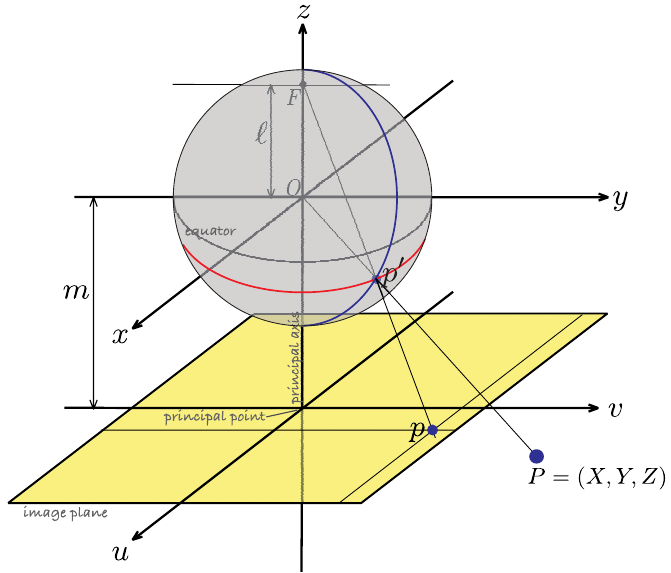
\includegraphics[width=.7\textwidth]{unified-im-model}
\caption{Geyer and Daniilidis (2000)}
\end{figure}
\end{frame}

\begin{frame}
\[
r = \dfrac{(l+m)\sin \theta}{l + \cos \theta}
\]
\begin{itemize}
\item It has two parameters $m$ and $l$.
\item For a perspective camera, the two points $O$ and $F$ coincide.
\item For catadioptric cameras with mirrors that are conics the focus $F$ lies between the center
of the sphere and the north pole, that is, $0 < l < 1$.
\end{itemize}
\end{frame}

\begin{frame}
\begin{figure}[!h]
\centering
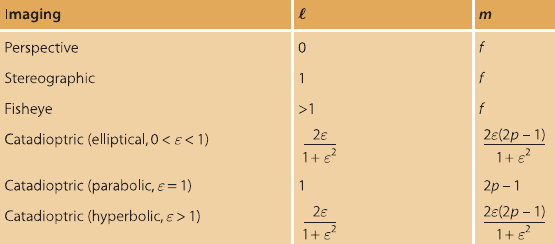
\includegraphics[width=.7\textwidth]{unified-imaging-table}
\end{figure}
\end{frame}

\begin{frame}[fragile]
From an image obtained with a fisheye lens to a ``pseudo''-spherical lens.
\begin{lstlisting}
fisheye = iread('fisheye_target.png', 'double', 'grey');
u0 = 528.1214; v0 = 384.0784;
l=2.7899;
m=996.4617;
[Ui,Vi] = imeshgrid(fisheye);
n = 500;
theta_range = (0:n)/n*pi/2 + pi/2;
phi_range = (-n:2:n)/n*pi;
[Phi,Theta] = meshgrid(phi_range, theta_range);
r = (l+m)*sin(Theta) ./ (l+cos(Theta));
U = r.*cos(Phi) + u0;
V = r.*sin(Phi) + v0;
spherical = interp2(Ui, Vi, fisheye, U, V);
idisp(spherical)
\end{lstlisting}
\end{frame}

\begin{frame}
\begin{figure}[!h]
\centering
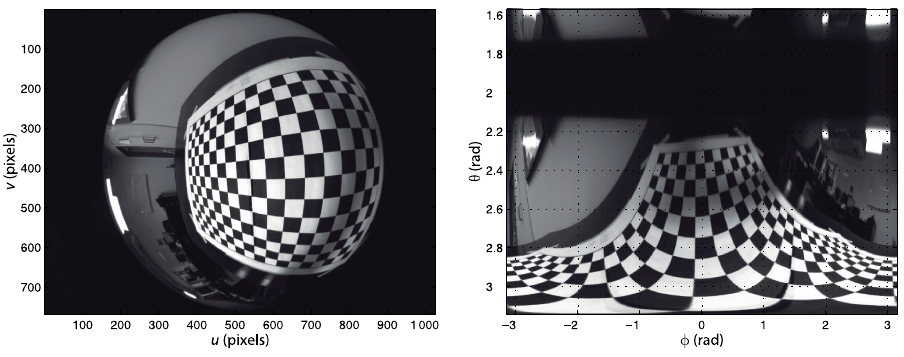
\includegraphics[width=\textwidth]{fig-11-23}
\end{figure}
\end{frame}

\begin{frame}[fragile]
\begin{lstlisting}
sphere_paint(spherical, 'south')
\end{lstlisting}
\begin{figure}[!h]
\centering
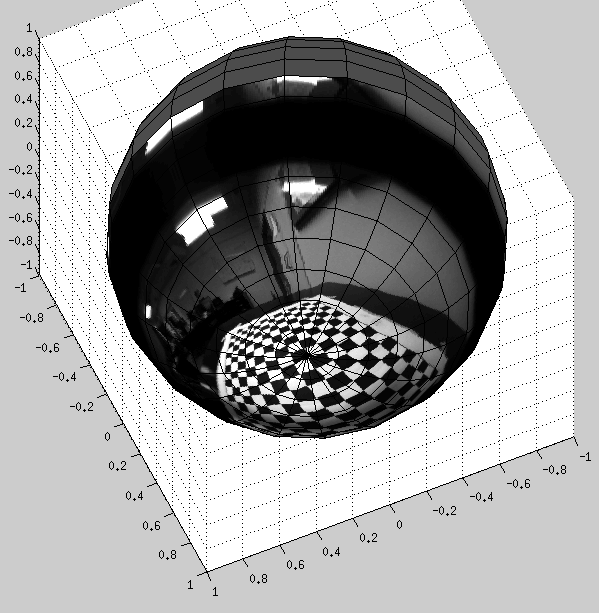
\includegraphics[width=.7\textwidth]{sphere}
\end{figure}
\end{frame}


%%%%%%%%%%%%%%%%%%%%%%%%%%%%%%%%%%%%%%%%%%%%%%%%%%%%%%%%%%%%%%%%%%%%%%%%%%%%%%%%%%%%%%%%%%%%%%%%%%%%%%%%%%%%%%%%%%%%%%%%%%%%%


\begin{frame}
\frametitle{Summary}
\begin{itemize}
\item Mapping points from 3D (world) to 2D (image) is achieved by a matrix multiplaction in homogeneneous coordinates.
\item Homogeneous coordinates are scale invariant.
\item Mapping points from one plane to another is achieved by a matrix multiplication with the planar homography matrix.
\end{itemize}
\end{frame}

%%%%%%%%%%%%%%%%%%%%%%%%%%%%%%%%%%%%%%%%%%%%%%%%%%%%%%%%%%%%%%%%%%%%%%%%%%%%%%%%%%%%%%%%%%%%%%%%%%%%%%%%%%%%%%%%%%%%%%%%%%%%%

%\section{References}
%
%\begin{frame}
%\frametitle{References}
%\begin{enumerate}
%\item Cork, P., ``\textit{Robotics, Vision and Control.}''. Springer, 2011.
%\end{enumerate}
%\end{frame}

\begin{frame}
\frametitle[alignment=center]{}
\flushbottom
\centering
Thank you!\\
\href{mailto:tiago@ic.ufal.br}{tvieira@ic.ufal.br}\\
%\href{mailto:warley.barbosa@edge.ufal.br}{warley.barbosa@edge.ufal.br}\\
%\href{mailto:icaro.bastos@edge.ufal.br}{icaro.bastos@edge.ufal.br}\\
\end{frame}


\end{document}